\section{Multi-arm Bandits}

RL evaluates the actions taken rather than instructs correct actions like other forms of learning.

\subsection{An n-Armed Bandit Problem}
\textbf{The problem}
\begin{itemize}
\item You are faced repeatedly with a choice of \textit{n} actions.
\item After each choice, you receive a reward from a stationary probability distribution.
\item Objective is to maximise total reward over some time period, say 100 time steps.
\item Named after of slot machine (one-armed bandit problem), but \textit{n} levers instead of 1.
\item Each action has an expected or mean reward based on its probability distribution. We shall call thjs the \textit{value} of the action. We do not know these values with certainty.
\item Because of this uncertainty, there is always an exploration vs exploitation problem. We always have one action that we deem to be most valuable at any instant, but it is highly likely, at least initially, that there are actions we are yet to explore that are more valuable.
\end{itemize}

\subsection{Action-Value Methods}
The estimated action value is
\begin{equation} \label{eq: estimated value}
	Q_t(a) = \frac{R_1+R_2+\cdots+R_{N_t(a)}}{N_t(a)}
\end{equation}

The true value (mean reward) of an action is \(q\), but the estimated value at the \textit{t}th time-step is Q(a), given by Equation \ref{eq: estimated value} (our estimate after \textit{N} selections of an action yielding \textit{N} rewards).\\

The greedy action selection method is
\begin{equation} \label{eq: argmax}
A_t =\argmax_a Q_t(a)
\end{equation}

\begin{itemize}
	\item Simplest action selection rule is to select the action with the highest estimated value.
	\item $\argmax_a$ means the value of \(a\) for which \(Q_t\) is maximised.
	\item \(\epsilon\)-greedy methods are where the agent selects the greedy option most of the time, and selects a random action with probability \(\epsilon\).
	\item Three algorithms are tried: one with \(e\)=0 (pure greedy), one with \(e\)=0.01 and another with \(e\)=0.1
	\item Greedy method gets stuck performing sub-optimal actions.
	\item \(e\)=0.1 explores more and usually finds the optimal action earlier, but never selects it more that 91\% of the time.
	\item \(e\)=0.01 method improves more slowly, but eventually performs better than the e=0.1 method on both performance measures.
	\item It is possible to reduce \(e\) over time to try to get the best of both high and low values.
\end{itemize}
\begin{figure}
	\centering
	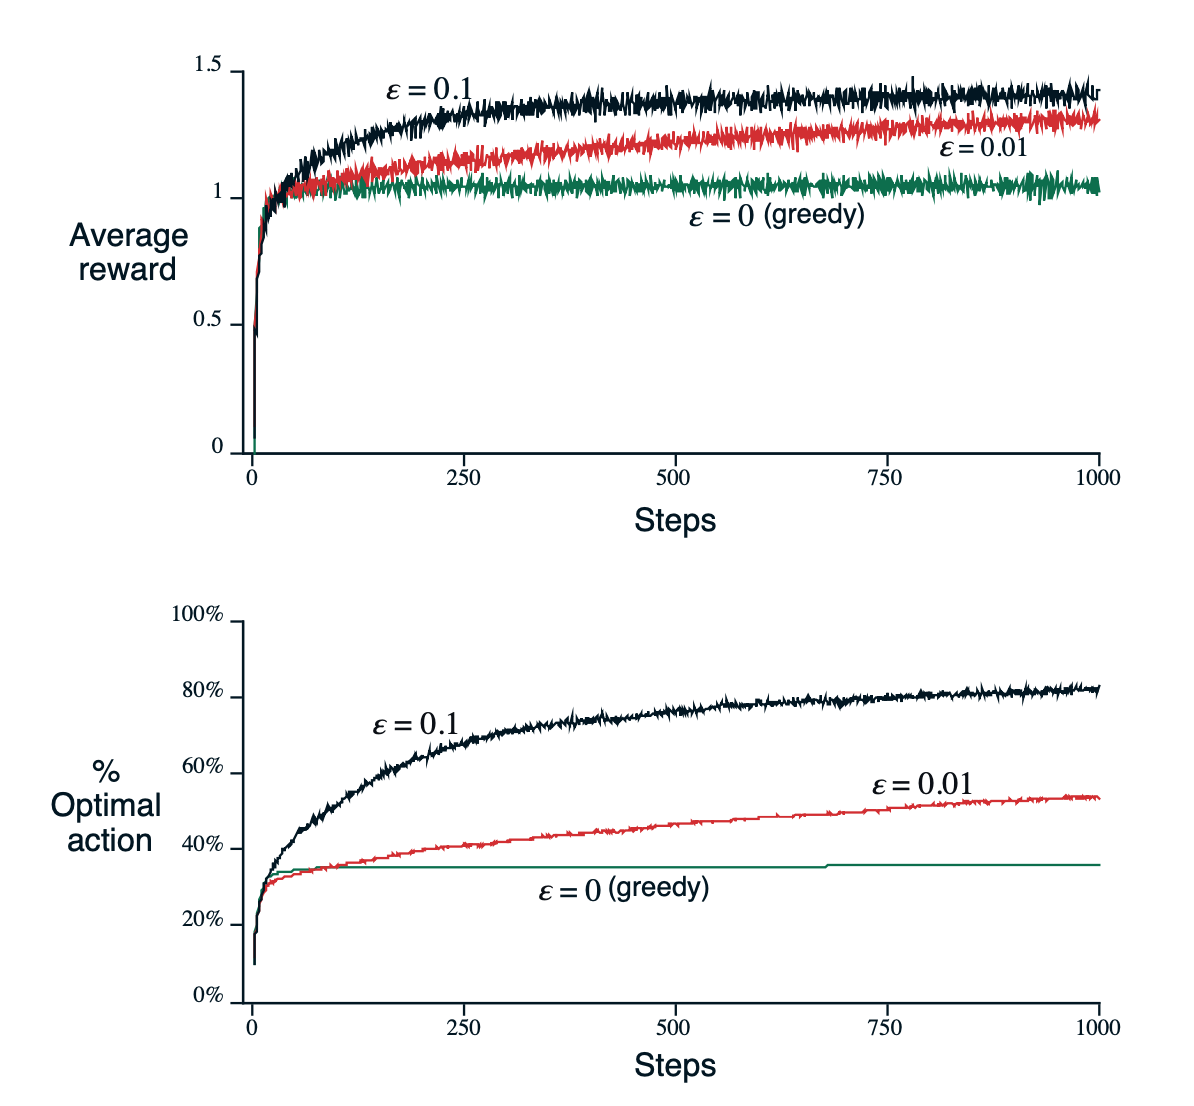
\includegraphics[width=0.8\textwidth]{/chapter2_1}
	\caption{Average performance of $\epsilon$-greedy action-value methods on the 10-armed testbed. These data are averages over 2000 runs with different bandit problems. All methods used sample averages as their action-value estimates.}
	\label{fig:chapter2_1}
\end{figure}

\subsection{Incremental Implementation}
The sample-average technique used to estimate action-values above has a problem: memory and computation requirements grow over time. This isn't necessary, we can devise an incremental solution instead:

\begin{align}
	Q_{k+1} &= \frac{1}{k}\sum_{i}^{k}R_i \nonumber \\
	&= \frac{1}{k} \left( R_k + \sum_{i=1}^{k-1} R_i \right) \nonumber \\
	&= \vdots \\
	&= Q_k + \frac{1}{k} \left[R_k - Q_k\right] \\
\end{align}

We are updating our estimate of \(Q_{k+1}\) by adding the discounted error between the reward just received and our estimate for that reward \(Q_k\).

\begin{equation}
NewEstimate \leftarrow OldEstimate + StepSize \left[Target - OldEstimate \right]
\end{equation}

\(\alpha\) is used to denote the stepsize (\(\frac{1}{k}\)) in the rest of this book.

\subsection{Tracking a Nonstationary Problem}
The averaging methods discussed above do not work if the bandit is changing over time. In such cases it makes sense to weight recent rewards higher than long-past ones. The popular way of doing this is by using a constant step-size parameter.

\begin{equation}
	Q_{k+1} = Q_k +\alpha \left[R_k - Q_k\right]
\end{equation}

where the step-size parameter \(\alpha \in (0,1]\) is constant. This results in \(Q_{k+1}\) being a weighted average of the past rewards and the initial estimate \(Q_1\):

\begin{align}
Q_{k+1} &= Q_k +\alpha \left[R_k - Q_k\right] \nonumber \\
&= \alpha R_k + (1 - \alpha)Q_k \nonumber \\
&= \alpha R_k + (1 - \alpha)[\alpha R_{k-1} + (1 - \alpha)Q_{k-1}] \nonumber \\
&= \alpha R_k + (1 - \alpha)\alpha R_{k-1} + (1 - \alpha)^2 Q_{k-1}  \nonumber \\
&= \vdots \nonumber \\
&= (1-\alpha)^k Q_1 + \sum_{i}^{k} \alpha (1 - \alpha)^{k-i} R_i \\
\end{align}

\begin{itemize}
\item Because the weight given to each reward depends on how many rewards ago it was observed, we can see that more recent rewards are given more weight. Note the weights \(\alpha\) sum to 1 here, ensuring it is indeed a weighted average where more weight is allocated to recent rewards.
\item In fact, the weight given to each reward decays exponentially into the past. This sometimes called an \textit{exponential} or \textit{recency-weighted} average.
\end{itemize}

\subsection{Optimistic Initial Values}
\begin{itemize}
\item The methods discussed so far are dependent to some extent on the initial action-value estimate i.e. they are biased by their initial estimates.
\item For methods with constant \(\alpha\) this bias is permanent.
\item In effect, the initial estimates become a set of parameters for the model that must be picked by the user.
\item In the above problem, by setting initial values to +5 rather than 0 we encourage exploration, even in the greedy case. The agent will almost always be disappointed with it's samples because they are less than the initial estimate and so will explore elsewhere until the values converge.
\item The above method of exploration is called \textit{Optimistic Initial Values}.
\end{itemize}

\subsection{Upper-confidence-bound Action Selection}
\(\epsilon\)-greedy action selection forces the agent to explore new actions, but it does so indiscriminately. It would be better to select among non-greedy actions according to their potential for actually being optimal, taking into account both how close their estimates are to being maximal and the uncertainty in those estimates. One way to do this is to select actions as:

\begin{equation}
	A_t = \argmax_a \left[Q_t(a) + c\sqrt{\frac{\ln t}{N_t(a)}}\right]
\end{equation}

where c \(>\) 0 controls the degree of exploration.

\begin{itemize}
	\item The square root term is a measure of the uncertainity in our estimate. It is proportional to \(t\) i.e. how many timesteps have passed and inversely proportional to \(N_t(a)\) i.e. how many times that action has been visited. The more time has passed, and the less we have sampled an action, the higher our upper-confidence-bound.
	\item As the timesteps increases, the denominator dominates the numerator as the ln term flattens.
	\item Each time we select an action our uncertainty decreases because N is the denominator of this equation.
	\item UCB will often perform better than e-greedy methods
\end{itemize}

\begin{figure}
	\centering
	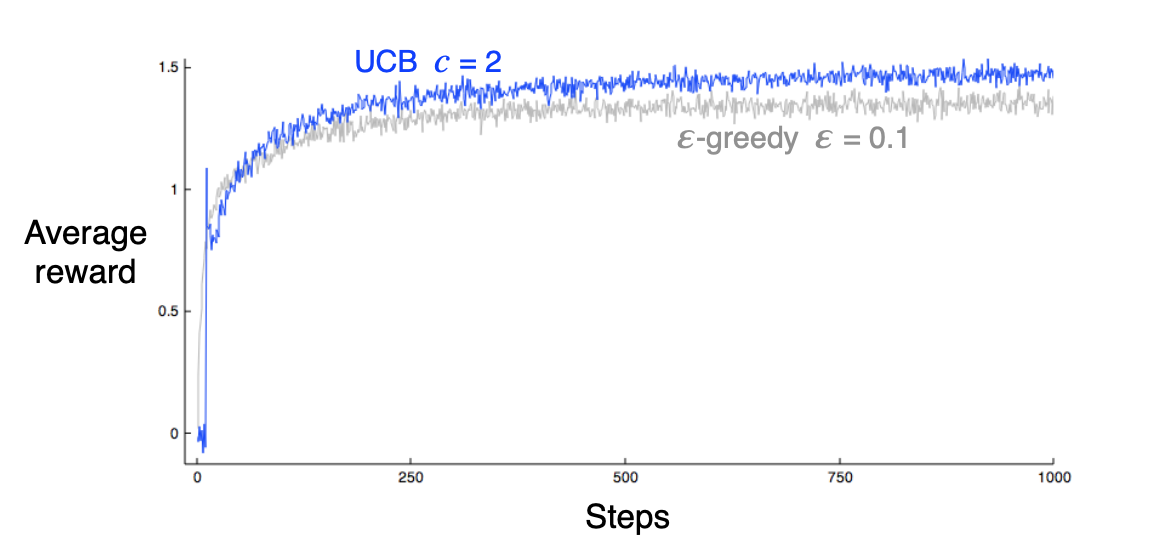
\includegraphics[width=0.8\textwidth]{/chapter2_2}
	\caption{UCB performs better than \(e\)-greedy in the n-armed bandit problem}
	\label{fig:chapter2_2}
\end{figure}

\subsection{Associative Search (Contextual Bandits)}
Thus far we have been discussing the stationary $k$-armed bandit problem, where the value of each arm is unknown but nonetheless remains stationary. Now, we consider a problem where the task could change from step to step, but the value distributions of the arms in each task remain the same. This is called contextual bandits, and in the toy example we are usually given a hint that the task has changed e.g. the slot machine changes colour for each task. Now we want to learn the correct action to take in a particular setting, given the task colour observed. This is an intermediary between the stationary problem and the full reinforcement learning problem. See exercise 2.10 below.

\subsection{Key Takeaways}
\begin{itemize}
\item The value of an action can be summarised by \(Q_t(a)\), the sample average return from an action
\item When selecting an action, it is preferable to maintain exploration, rather than only selecting the action we believe to be most valuable at any given timestep, to ensure we continue to improve our best estimate of the optimal action. We do so using \(\epsilon\))-greedy policies.
\item If our problem is non-stationary, rather than taking a standard average of every return received after an action, we can take a weighted average that gives higher value to more recently acquired rewards. We call this an \textit{exponential} or \textit{recency-weighted} average.
\item Optimistic initial values encourage lots of early exploration as our returns always decrease our estimate of \(Q_t\) meaning the greedy actions remain exploratory. Only useful for stationary problems.
\item \(\epsilon\)-greedy policies can be adapted to give more value to actions that have been selected less-often, i.e. actions where we have higher uncertainty in their value, using \textit{upper-confidence-bound} action selection.
\item Lastly, each of these techniques have varied performance on the n-armed bandit test dependent on their parametrisation. Their performance is plotted in Figure \ref{fig:chapter2_4}.
\end{itemize}

\begin{figure}
	\centering
	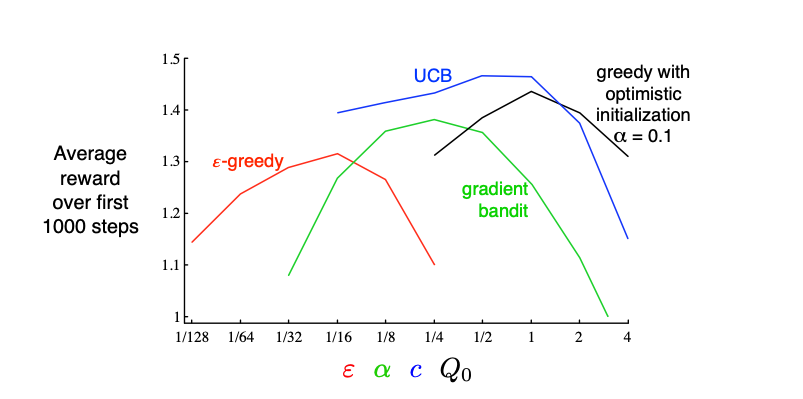
\includegraphics[width=0.8\textwidth]{/chapter2_4}
	\caption{Performance of each of the bandit algorithms explored in this chapter}
	\label{fig:chapter2_4}
\end{figure}

